\clearpage
\setcounter{page}{1}
\maketitlesupplementary
\appendix

% \section{Rationale}
% \label{sec:rationale}
% % 
% Having the supplementary compiled together with the main paper means that:
% % 
% \begin{itemize}
% \item The supplementary can back-reference sections of the main paper, for example, we can refer to \cref{sec:intro};
% \item The main paper can forward reference sub-sections within the supplementary explicitly (e.g. referring to a particular experiment); 
% \item When submitted to arXiv, the supplementary will already included at the end of the paper.
% \end{itemize}
% % 
% To split the supplementary pages from the main paper, you can use \href{https://support.apple.com/en-ca/guide/preview/prvw11793/mac#:~:text=Delete%20a%20page%20from%20a,or%20choose%20Edit%20%3E%20Delete).}{Preview (on macOS)}, \href{https://www.adobe.com/acrobat/how-to/delete-pages-from-pdf.html#:~:text=Choose%20%E2%80%9CTools%E2%80%9D%20%3E%20%E2%80%9COrganize,or%20pages%20from%20the%20file.}{Adobe Acrobat} (on all OSs), as well as \href{https://superuser.com/questions/517986/is-it-possible-to-delete-some-pages-of-a-pdf-document}{command line tools}.

% \begin{table}[t]
%     \centering
%     \vspace{0pt} % Ensures top alignment
%     \resizebox{\linewidth}{!}{%
%    \input{./tables/ablation_reconstruction_targets} 
%     }
%     \caption{\textbf{Reconstruction targets.}  Reconstruction targets including both the original frame and the next or precious frames do better than reconstruction targets incorporating information from just one. Reconstruction targets with the current frame backed in have *. All results are on CNNs with resolution 1024 and bottleneck 512 and no skip connections.}
% \label{tab:ablation_reconstruction_targets}
% \end{table}

We present additional experimental results as ablations Sec.\ (\ref{sec:ablations}), additional implementation details (Sec.\ \ref{sec:implementation_deets}), and additional visualizations (Sec.\ \ref{sec:visualizations}).

\textbf{Benefits and risks of this technology}. Improving classification, tracking, and counting in sonar and ultrasound videos is useful across medical, ecological, and other fields. Counting fish with sonar allows for a non-invasive way to measure population size, which can then be used for conservation and ecological efforts, for understanding effects of climate change, and for monitoring human fishing behavior for economical reasons. Improving classification in ultrasound videos, too, paves a path for more automated diagnosis. Risks, though, are inherent in both tracking applications and applications of sensitive data. Care must be taken when using these models, so that they are not used blindly without human intervention to make decisions.

\section{Additional Experimental Results}\label{sec:ablations}

\subsection{Additional CFC22 Ablation Results}\label{sec:ablation_additions}

As in the main paper, we evaluate CFC22 on the detection val/test splits, and show results using mAP$_{50}$ across the dataset splits. We look at the effect of bottleneck size in the hourglass network, traditional augmentations, input resolution size, and reconstruction targets on how the trained denoiser affects downstream detection performance. We also look at the effect of downstream task performance when using the reconstruction target alone ($S_{t,T}$) compared with using the learned reconstruction ($\hat{S}_{t,T}$).

\textbf{Bottlenecks size}. For all experiments on CFC22, we use a default input size of 1024hx512w, reconstruction target as PFDwT1, mean-squared error (MSE) loss, and we train the denoiser for 20 epochs. Here the hourglass network remains 2 layers, with the number of input channels as 512, but the number of channels in the middle layer changes. We notice that for training, larger (less-restrictive) bottlenecks yield higher performance. For val and test, though, bottleneck sizes over 64 improve performance, but the differences between 128 and 512 is worse for val and negligible for test. Results can be seen in \cref{tab:bottleneck}.

\textbf{Resolution size}. We vary the input resolution size to train the denoiser and notice higher performance for train and test when higher resolutions are used, seen in \cref{tab:resolution}. We hypothesized that higher resolution size would make the denoiser more stable for downstream detections because higher resolution sizes would mean that removing entire fish (\ie small fish) would be less probable. It is interesting to note that the highest resolution size 2048x1024 for val led to lower detection performance than that of resolution size 1024x512. We note, though, that higher resolutions lead to smaller batch sizes and longer training time.

\textbf{Traditional Augmentations}. We apply salt-and-pepper noise, gaussian-blur, motion-blur, brightness, and erasing from the kornia.Augmentations library. We apply these augmentations when training the denoiser. We do \textit{not} apply these augmentations when training downstream tasks. We found that no traditional augmentations to train the denoiser, though, improve downstream performance. Results can be seen in \cref{tab:augmentations}.
%These augmentations are commonly used \CITE{} as ways to make training robust to unpredictably noisy imagery. 

\textbf{Reconstruction Targets}. We experimented with a handful of reconstruction targets: 

\textit{Frame difference}---such as absolute difference ($S_{|d|}=|I_t - I_{t+T}|$) or raw difference ($S_d=I_t - I_{t+T}$)---has been used in other self-supervised works as a spatiotemporal reconstruction target \cite{sun2022bkind}. This works well in video where the movement in the background is less than the foreground movement. For our experiments, we use absolute difference as frame difference.

\textit{Raw frame} ($I_t$) predicts the input (identity) frame alone.

\textit{Background subtraction} (bs) We approximate the background frame,  $\bar{I_v}$, as the mean aggregate of video over time. This is based on the approximation that objects of interest are sparse in terms of space and time. The mean frame is subtracted from every frame in the video ($S_d=(I_{v})_t - \bar{I_v})$. 

\textit{Positive Frame Difference with current frame} (PFDwTN). We discuss this in more detail in the main paper, \cref{sec:reconstruction}. We experimented with T=2 (PFDwT2) and T=1 (PFDwT1), ultimately selecting T=1. 

\textit{Standard Deviation across all frames} ($\sigma$) is taken across all of the frames loaded in a window of continuous frames, $\sigma(I_{t-N}:I_{t+N})$ where 2N+1 is the size of the window. We experimented with N=1 and N=2.

\textit{Sum frames minus N*background} ($\Sigma-N\bar{I_v}$) sums all of the frames in a window size N and takes the positive difference $N*\bar{I_v}$ where $\bar{I_v}$ is the mean frame of all frames in a video: $\max(0, (\sum_t^{T}I_t) - N\bar{I_v})$. We experimented with window sizes N=3 and N=5.

Visualizations of all of these can be seen in \cref{fig:reconstruction_targets_supp}

\begin{table}[t]
\centering
\vspace{0pt} % Ensures top alignment
% \resizebox{0.9\linewidth}{!}{%
\begin{tabular}{lcccc}
 \toprule
 & & \multicolumn{3}{c}{mAP$_{50}$} \\
 \cmidrule(r){3-5}
\multicolumn{1}{c}{Signal Modification} & \multicolumn{1}{c}{AE} & \multicolumn{1}{c}{Train} & \multicolumn{1}{c}{Val} & \multicolumn{1}{c}{Test} \\
\midrule
% Option A\\
% \midrule
% Raw ($I_t$) & \xmark &  &  &   \\ 
% Raw ($I_t$) \MAH{Check this} & \cmark & 81.5  & 68.4 & 73.4 \\
% $\sigma$ & \xmark & 79.8 & 69.4 & 72.5  \\ 
% $\sigma$ & \cmark &  &  &   \\
% $\Sigma-5\bar{I}$ & \xmark & 78.3 & 67.6 &  71.17 \\ 
% $\Sigma-5\bar{I}$ \MAH{Check this} & \cmark & 78.8 & 69.2 &  72.8\\
% PFDwT1 & \xmark & 80.2 & 66.9 & 68.2\\ 
% PFDwT1 & \cmark &  & 70.6 & 77.6 \\
% PFDwT2 & \xmark & 81.2 & 68.1 &  63.0 \\ 
% PFDwT2  & \cmark & & & \\
% \bottomrule
% \\
% Option B\\
% \\
 \toprule
\multicolumn{5}{l}{\textit{Signal Modification w/o Denoising Network}}\\
Raw ($I_t$) & \xmark & 79.6 & 69.6 & 54.2  \\ 
$\sigma$ & \xmark & 79.8 & 69.4 & 72.5  \\ 
$\Sigma-5\bar{I}$ & \xmark & 78.3 & 67.6 &  71.7 \\ 
PFDwT1 & \xmark & 80.2 & 66.9 & 68.2\\ 
PFDwT2 & \xmark & 81.2 & 68.1 &  63.0 \\ 
\multicolumn{5}{l}{\textit{Signal Modification w/ Denoising Network}}\\
Raw ($I_t$) & \cmark & 81.5  & 68.4 & 73.4 \\
$\sigma$ & \cmark & 82.2 & 70.0 & 73.5  \\
$\Sigma-5\bar{I}$ & \cmark & 79.8 & 68.1 &  71.7 \\
\rowcolor{lightgray}
PFDwT1 & \cmark & \textbf{83.5} & \textbf{70.6} & \textbf{77.6} \\
PFDwT2  & \cmark & 82.2 & 68.5 & 71.4 \\
\bottomrule
\end{tabular}

%}
\caption{\textbf{Effect of Different Motion Enhancements with and without \NAME{}'s Autoencoder Network (AE) on CFC22.} All detectors that leverage the AE have superior performance to those that use only the motion-enhanced target on the test set. The modified signal is used as the reconstruction target for the denoising autencoder when it is present, and is the input signal for the downstream task when the autoencoder is not used. All results are on CNNs with skip connections with resolution 1024 and bottleneck 512.}
\label{tab:ablation_reconstruction_targets}
\end{table}

\captionsetup{font=small}
\begin{figure*}[p]
    \centering
    \begin{subfigure}[b]{0.5\linewidth}
        \centering
        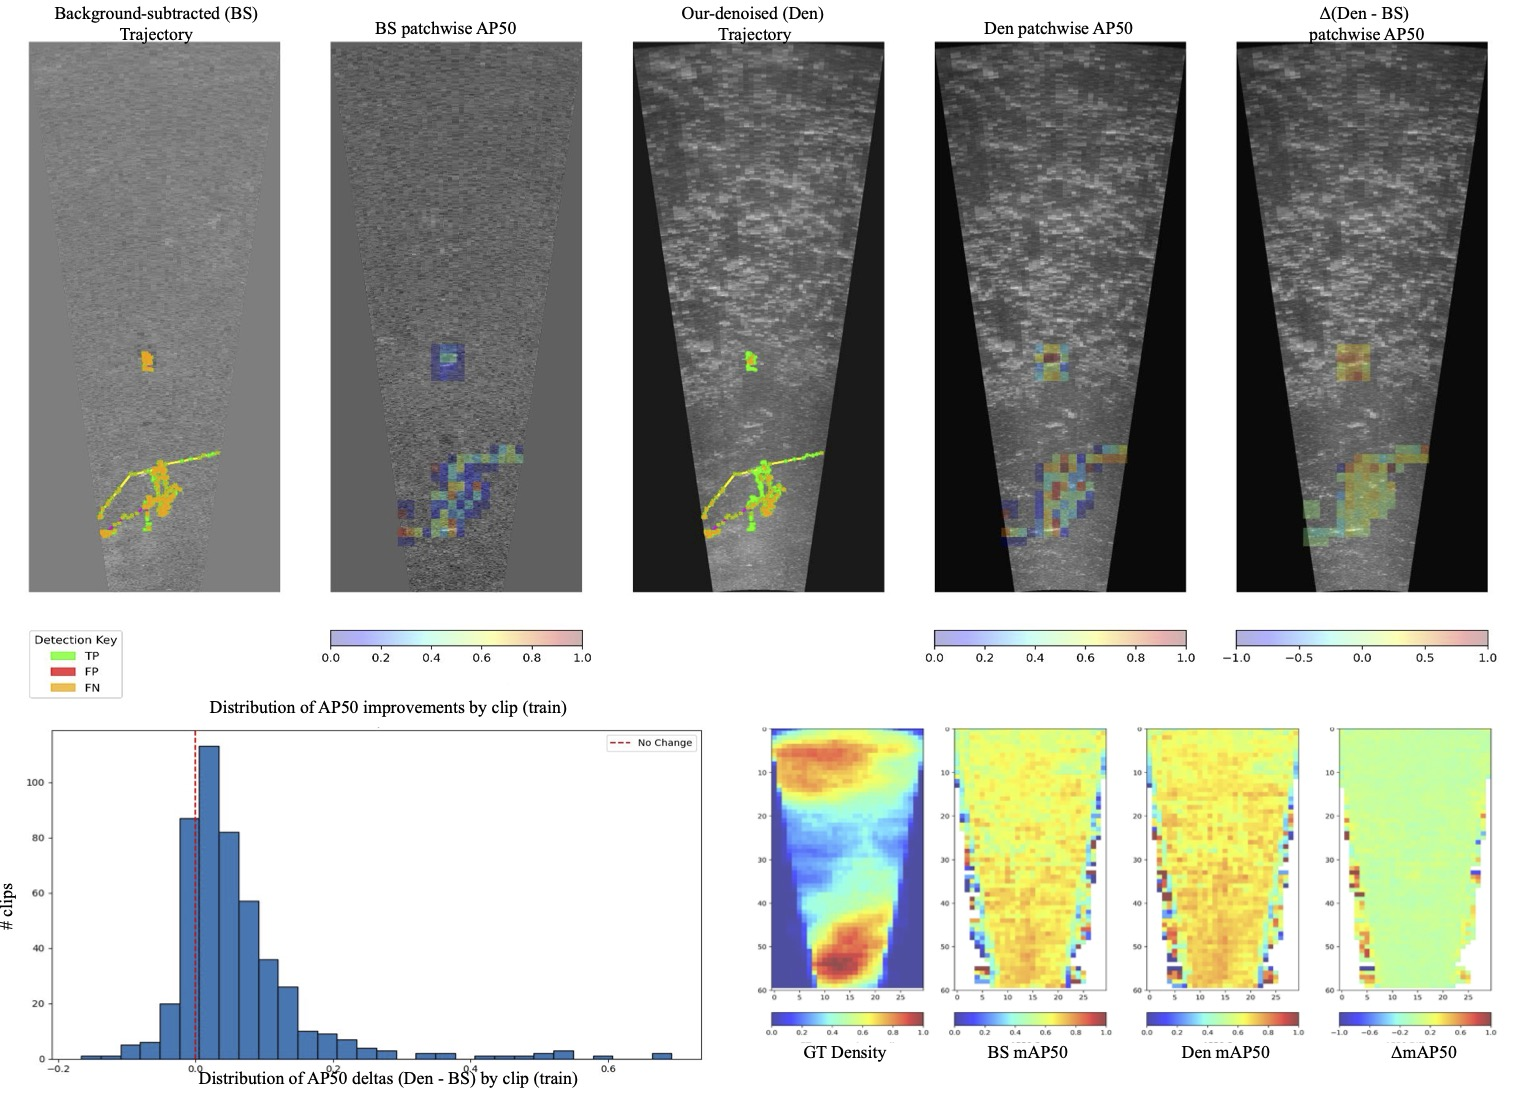
\includegraphics[width=0.95\linewidth]{figs/train_trajectory_example.jpg}
        \caption{One clip from the CFC22-train river. You can can see the trajectory and patchwise detection performance improves after denoising. Overall, the biggest denoising gains appear to be at the edges of the cone, where fish are known to be small (entering/exiting) but moving.}
        \label{fig:train_trajectory_example_with_detections}
    \end{subfigure}
    \hfill
    \quad
    \begin{subfigure}[b]{0.5\linewidth}
        \centering
        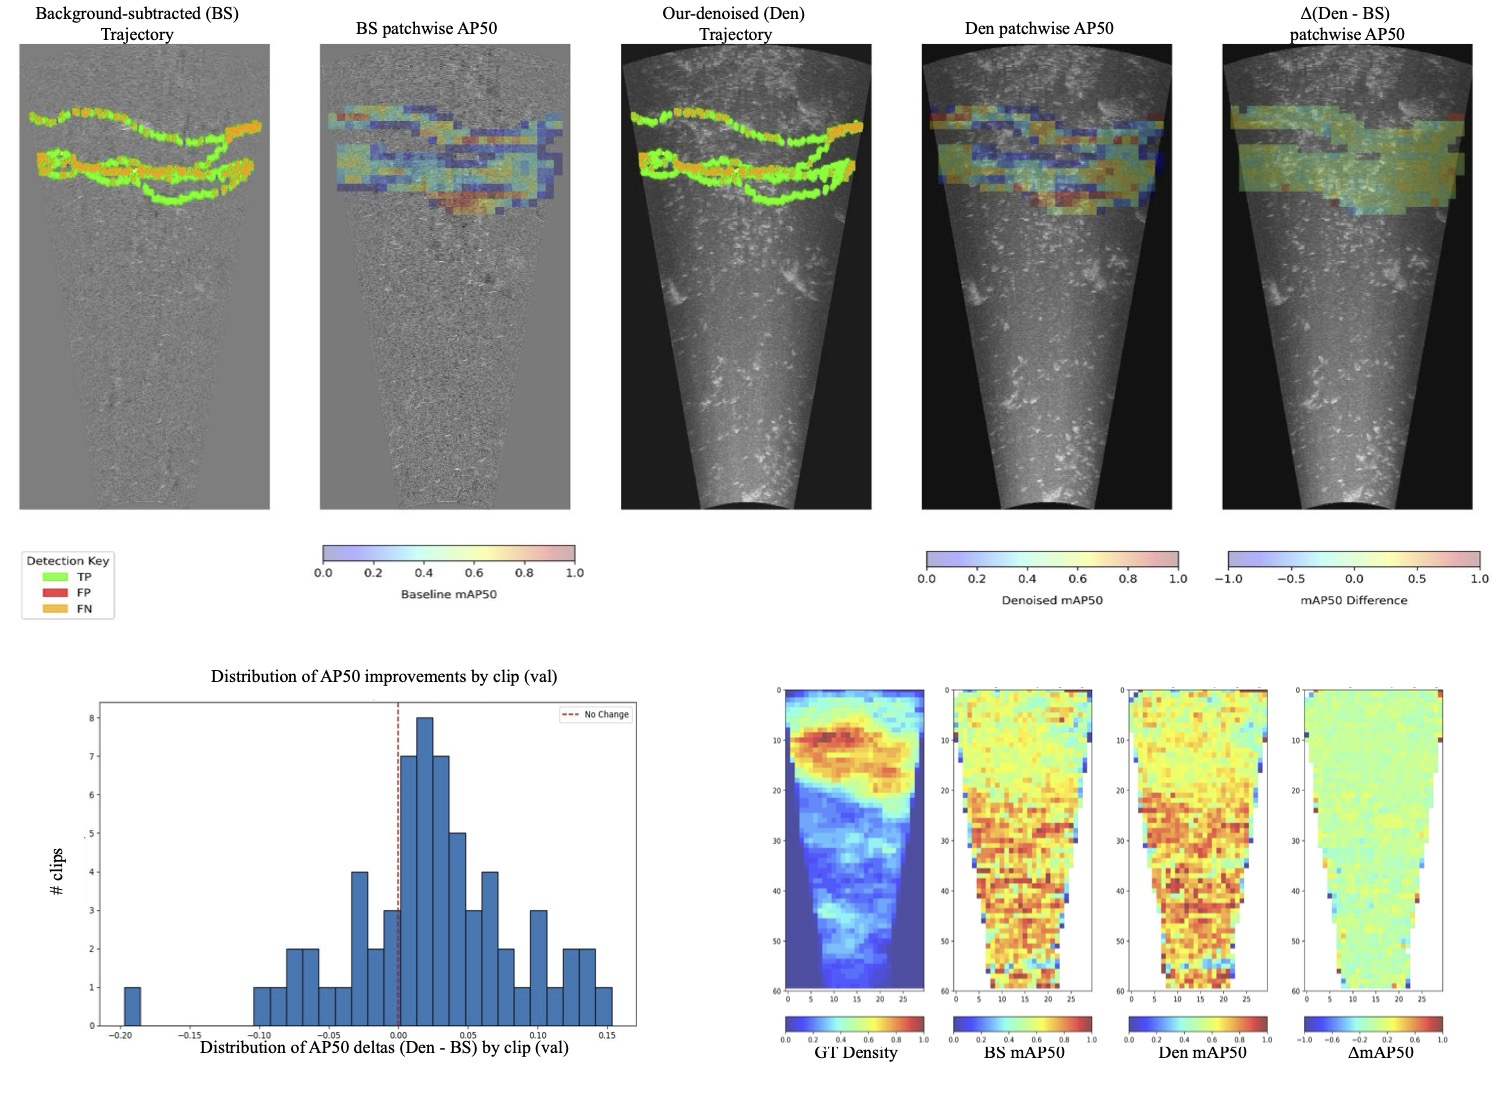
\includegraphics[width=0.95\linewidth]{figs/cfc22_val_track_and_det.jpg}
        \caption{One clip from the CFC22-val river. The denoising gain is smaller and therefore more difficult to see here.}
        \label{fig:val_trajectory_example_with_detections}
    \end{subfigure}
    \hfill
    \quad
    \begin{subfigure}[b]{0.5\linewidth}
        \centering
        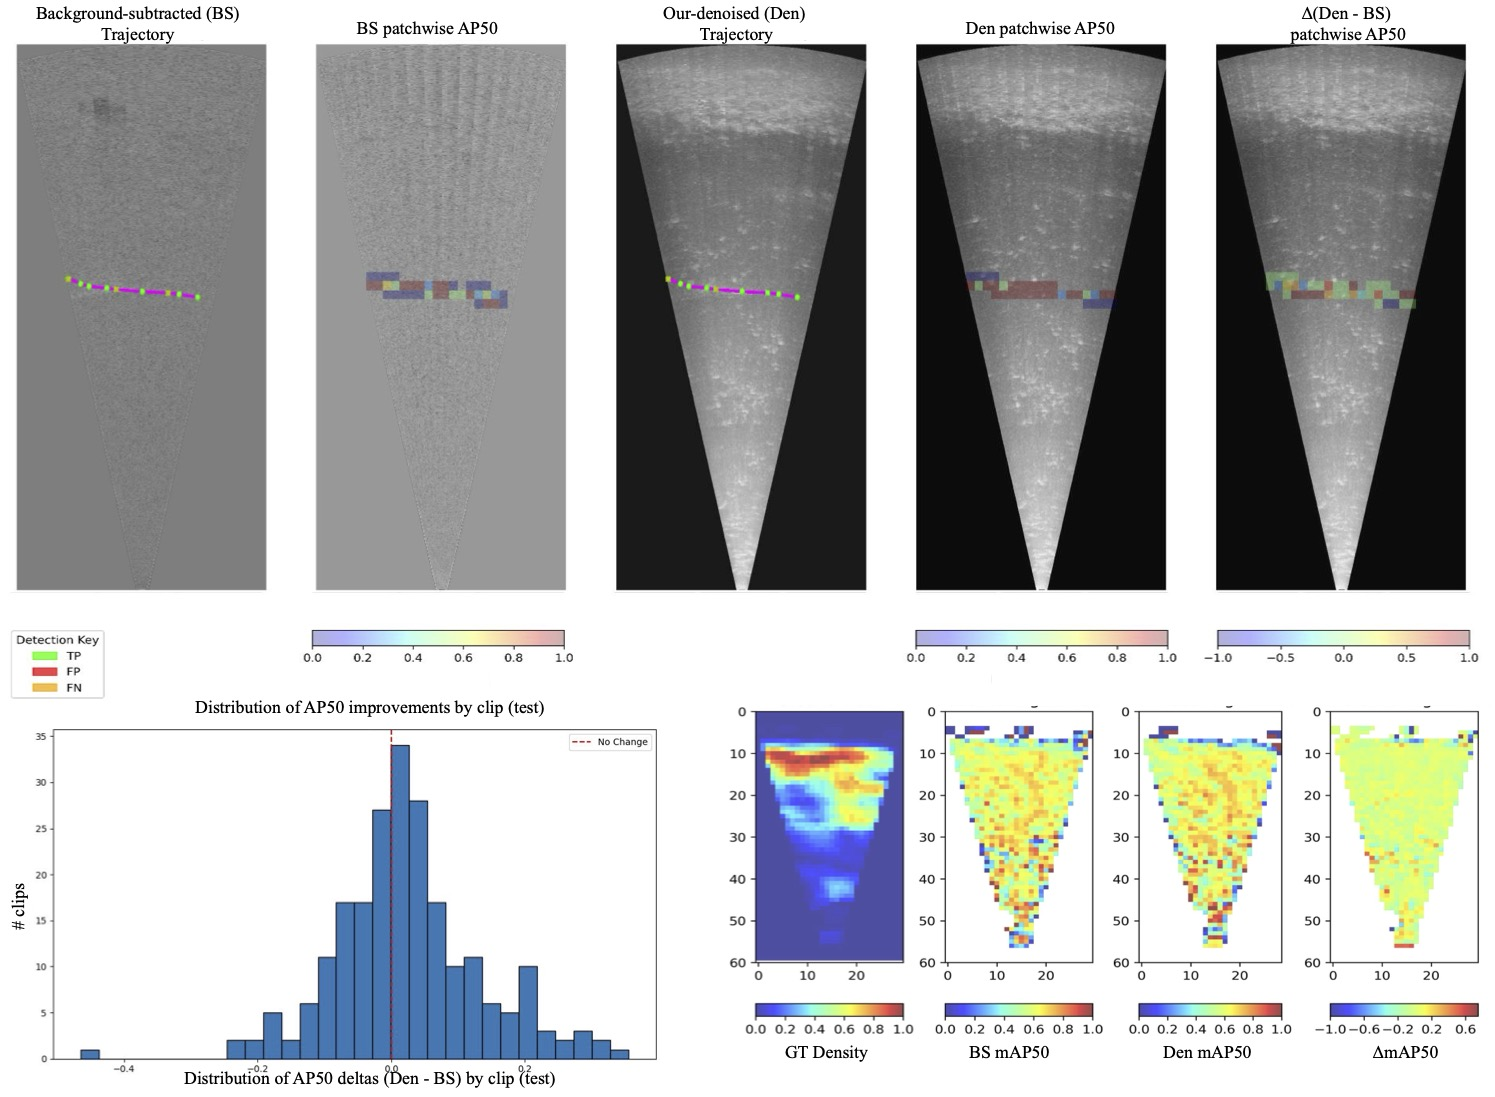
\includegraphics[width=0.95\linewidth]{figs/cfc22_test_track_and_det.jpg}
        \caption{One clip from the CFC22-test river.}
        \label{fig:test_trajectory_example_with_detections}
    \end{subfigure}
    \caption{\textbf{Denoising-improved detection leads to better tracks}. On the single-clip trajectory plots, orange dots indicate false negatives, green dots indicate true positives, red indicates false positives.}
    \label{fig:trajectory_example_with_detections}
\end{figure*}


\captionsetup{font=small}
\begin{figure*}[!htbp]
\centering
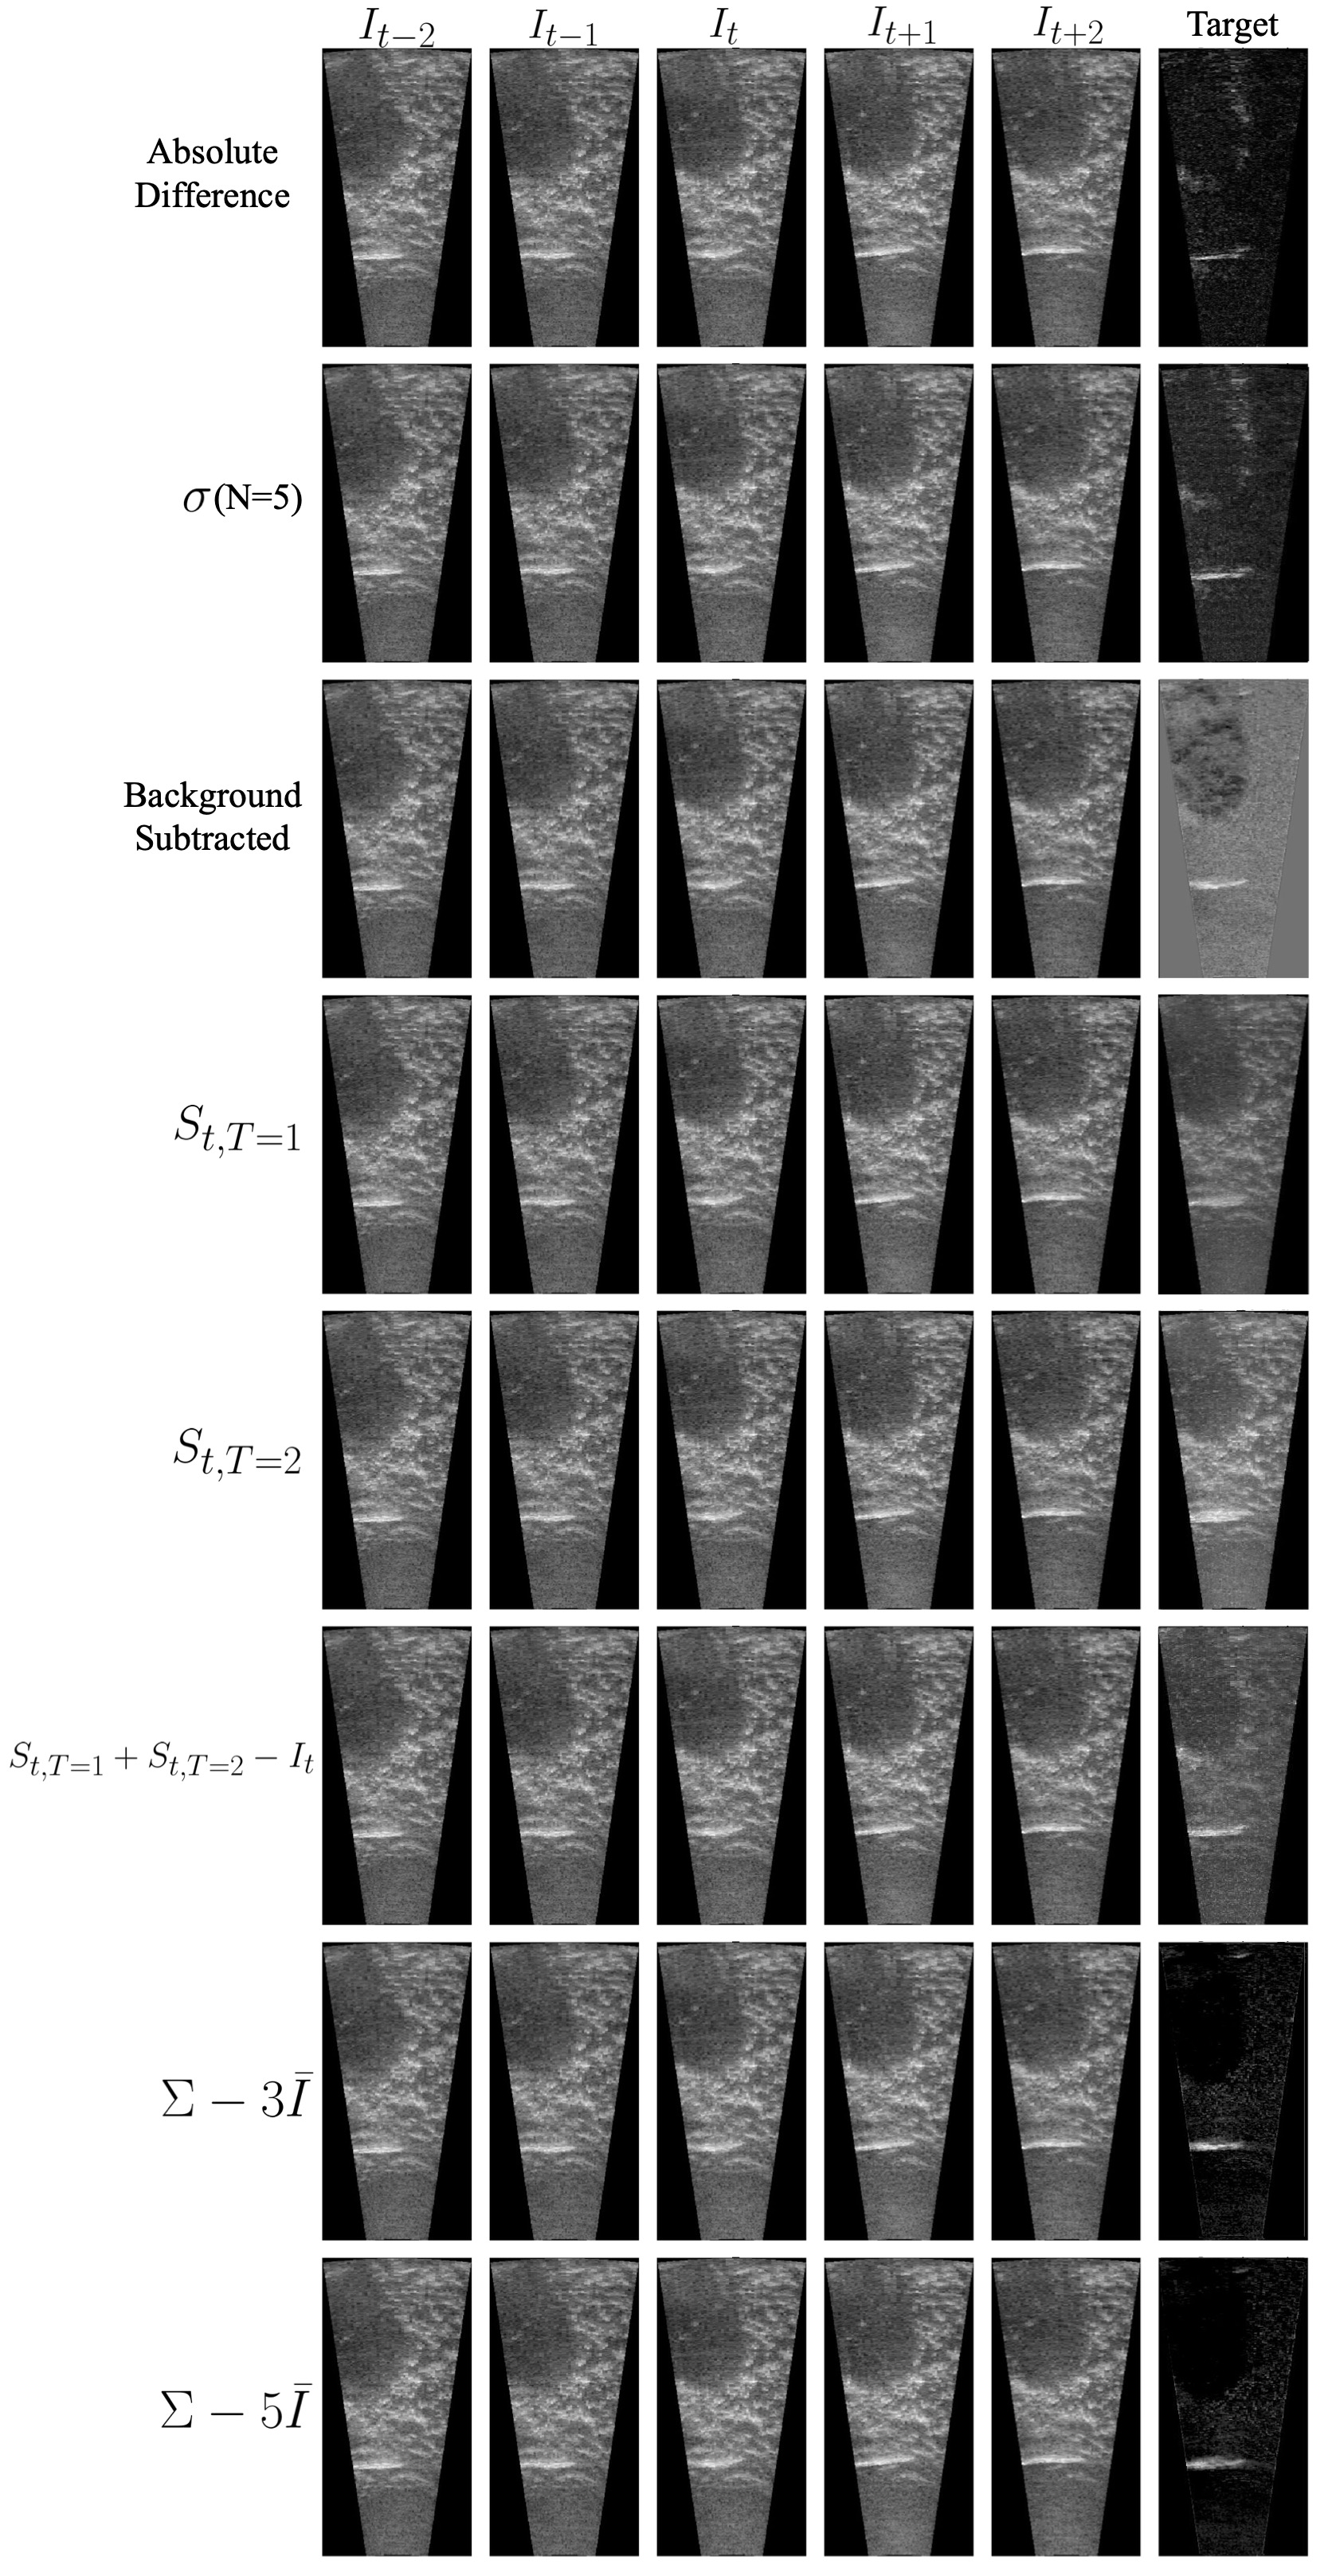
\includegraphics[width=0.5\linewidth]{figs/reconstruction_targets_supp.jpg}
\caption{\textbf{Reconstruction Targets}. The window T=5 set of frames is shown with each reconstruction target we experimented with on CFC22. While $\Sigma-N\bar{I}$ frames appear strong in this example, we found that empirically they struggled to capture fish that did not move significantly between frames.}
\label{fig:reconstruction_targets_supp}
\end{figure*}

\begin{table*}[bp]
\centering
\scriptsize
\begin{subtable}[t]{0.48\textwidth}
    \centering
    \vspace{0pt} % Ensures top alignment
    \begin{tabular}{c c c c}
    \toprule
    & \text{Train} & \text{Val} & \text{Test1} \\
    \text{Bottleneck} & \text{mAP$_{50}$} & \text{mAP$_{50}$} & \text{mAP$_{50}$} \\ 
    \hline
    %32 & - & - & - \\ 
    64 & 79.1 & 68.6 & 71.6 \\
    128 & 80.0 & 69.2 & \textbf{72.6} \\ 
    %256 & - & - & - \\
    \rowcolor{lightgray}
    512 & \textbf{81.6} & \textbf{69.4} & \textbf{72.6}\\
    \bottomrule
    \end{tabular}
    \caption{\textbf{Bottleneck size.} A larger bottleneck outperforms overly-constricted networks. All results are from CNNs with no skip connections and non-residual blocks.}
    \label{tab:bottleneck}
\end{subtable}\hfill
\quad
\begin{subtable}[t]{0.48\textwidth}
    \centering
    \vspace{0pt} % Ensures top alignment
    \begin{tabular}{c c c c}
    \toprule
    & \text{Train} & \text{Val} & \text{Test1} \\
    \text{Resolution} & \text{mAP$_{50}$} & \text{mAP$_{50}$} & \text{mAP$_{50}$} \\ 
    \hline
    512 & \textbf{81.3} & \textbf{69.2} & 71.9 \\ 
    \rowcolor{lightgray}
    1024 & 79.1 & 68.6 & 71.6 \\
    2048 & 80.1 & 68.1 & \textbf{72.1} \\ 
    \bottomrule
    \end{tabular}
    \caption{\textbf{Resolution size.} There is no clear optimal - in terms of train and val, the smallest resolution size is the best; however, in terms of test, the largest resolution size is optimal. Note that higher resolutions also lead to longer training times.}
    \label{tab:resolution}
\end{subtable}\hfill
\quad
\begin{subtable}[t]{0.48\textwidth}
    \centering
    \vspace{0pt} % Ensures top alignment
    \begin{tabular}{l c c c}
    \toprule
    & \text{Train} & \text{Val} & \text{Test1} \\
    \text{Augmentations} & \text{mAP$_{50}$} & \text{mAP$_{50}$} & \text{mAP$_{50}$} \\ 
    \hline
    $\text{saltpepper}_{0.25}$ & 81.2 & 68.5 & 72.2 \\ 
    $\text{saltpepper}_{0.5}$ & \textbf{83.7} & 69.7 & 75.1 \\
    $\text{saltpepper}_{0.75}$ & 81.4 & 69.2 & 72.8 \\ 
    $\text{gaussianblur}_{0.25}$ & 82.1 & 69.9 & 74.8 \\
    $\text{gaussianblur}_{0.5}$ & 81.3 & 68.9 & 75.0 \\
    $\text{gaussianblur}_{0.75}$ & 83.5 & 68.4 & 75.6 \\
    $\text{motionblur}_{0.25}$ & 83.5  & 68.3 & 76.5 \\
    $\text{motionblur}_{0.5}$ & 81.2 & 68.2 & 74.7 \\
    $\text{motionblur}_{0.75}$ & \textbf{83.7} & 69.6 & 73.9\\
    $\text{brightness}_{0.25}$ & \textbf{83.7} & 69.8 & 74.7 \\
    $\text{brightness}_{0.5}$ & 82.2 & 69.0 & 73.9 \\
    $\text{brightness}_{0.75}$ & 83.6 & 69.7 & 76.8 \\
    $\text{erase}_{0.25}$ & 82.0 & 68.7 & 68.0 \\
    $\text{erase}_{0.5}$ & 81.1 & 68.7 & 75.6  \\
    $\text{erase}_{0.75}$ & 77.4 & 59.3 & 62.4 \\
    \rowcolor{lightgray}
    No augmentations & 83.5 & \textbf{70.6} & \textbf{77.6} \\
    \bottomrule
    \end{tabular}
    \caption{\textbf{Augmentations.} Augmentations appear to degrade performace. All augmentation experiments are named as $augmentation_{probability}$. All networks are CNNs with skip connections with resolution 1024 and bottleneck 512.}
    \label{tab:augmentations}
\end{subtable}\hfill
\quad
\begin{subtable}[t]{0.48\textwidth}
    \centering
    \vspace{0pt} % Ensures top alignment
    \begin{tabular}{l c c c}
    \toprule
    & \text{Train} & \text{Val} & \text{Test1} \\
    \text{Target} & \text{mAP$_{50}$} & \text{mAP$_{50}$} & \text{mAP$_{50}$} \\ 
    \hline
    Raw* & 81.5 & 68.4 & 73.4 \\
    Absolute Difference $|I_t - I_{t+1}|$ & 81.6 & 69.2 & 73.5 \\ 
    Sigma(N=5) & 78.8 & 69.2 & 72.8 \\
    \rowcolor{lightgray}
    $\hat{S}_{t,T=1}$* & 82.7 & 70.0 & 74.0 \\
    $\hat{S}_{t,T=2}$* & 82.8 & \textbf{70.6} & 73.0\\
    $\hat{S}_{t,T=2} + \hat{S}_{t,T=1} - I_t$* & \textbf{83.7} & 69.2 & \textbf{74.6} \\
    $\Sigma-3\bar{I}$ & 80.3 & 68.3 & 69.0\\
    $\Sigma-5\bar{I}$ & 80.7 & 68.7 & 72.0 \\ 

    \bottomrule
    \end{tabular}
    \caption{\textbf{Reconstruction targets.} Reconstruction targets including both the original frame and the next or previous frames do better than reconstruction targets incorporating information from just one. Reconstruction targets with the current frame in have *. All results are on CNNs with resolution 1024 and bottleneck 512 with no skip connection.}
    \label{tab:targets}
\end{subtable}\hfill

\begin{subtable}[t]{0.48\textwidth}
    \centering
    \vspace{0pt} % Ensures top alignment
    \begin{tabular}{lccc}
    \toprule
    & \text{Train} & \text{Val} & \text{Test1} \\
    \text{Architectures} & \text{mAP$_{50}$} & \text{mAP$_{50}$} & \text{mAP$_{50}$} \\ 
    \hline
    Autoencoder & 82.6 & 68.9 & 67.8 \\
    CNN-fine & 82.7 & 69.1 & 74.0 \\
    \rowcolor{lightgray}
    CNN-SKIP & \textbf{83.5} & \textbf{70.6} & \textbf{77.6} \\ 
    CNN-residual & \textbf{83.5} & 69.2 & 73.1 \\
    CNN-resnet-block & 79.8 & 70.0 & 73.6\\
    UNet-downscaled & 82.1 & 69.1 & 75.8 \\
    UNet & 81.2 & 70.0 & 73.9 \\
    UNet3D & 79.0 & 67.0 & 66.9\\
    \bottomrule
    \end{tabular}
    \caption{\textbf{Denoising backbone architecture.} All experiments have our target from equation 2 ($\hat{S}_{t,T=1}$) as their target. Networks are ordered from smallest (in terms of parameters and TFLOPs) to largest -- it is interesting to note that as model size increases, performance does not necessarily increase. We see the top performer is the CNN-SKIP architecture.}
    \label{tab:architecture}
\end{subtable}\hfill

\caption{\textbf{Additional denoise-detection ablations on CFC22.} All values are generated via the detection stage of our pipeline. All reconstruction targets are sized 1024 x 512 unless otherwise stated. We report the mAP$_{50}$ of the \emph{combined} background-subtracted and target reconstruction frame unless otherwise noted. Default settings are marked in \colorbox{lightgray}{gray}. }
\label{tab:additional_ablations}
\end{table*}
\vspace{1em}


% \begin{table}
%     \centering
%     \resizebox{\linewidth}{!}{%  
%     \begin{tabular}{lccccc}
%     \toprule
% Method & Hellinger $\uparrow$& IoU $\downarrow$ & KL $\uparrow$& Chi2 $\uparrow$& Wasserstein $\uparrow$\\
% \hline
% raw & 0.3431 & 0.5382 & 859.8 & 94.21 & 0.05574 \\
% $bs$ & 0.3383 & 0.5489 & 896.9 & 91.42 & 0.04096\\
% $bs_{3ch}$ &\textit{0.2608} &\textit{0.6377} &\textit{458} &\textit{58.17} &\textit{0.0365} \\
% $den$ &\textbf{0.4866} &\textbf{0.3717} & 548 & 172 & 0.07506 \\
% $den_{plus}$ &0.4569 & 0.4043 &\textbf{1458} &\textbf{157.3} &\textbf{0.08076} \\
% \bottomrule
%     \end{tabular}
%     }
%     \caption{\textbf{Denoised methods distance metrics between P (Fish) vs. Q (Non-fish) as distributions of pixel intensities.} For all ground truth bounding boxes, P and Q are composed as follows: P -- we take the set of pixels in the bounding box from the frame with the fish. Q -- we extract the set of pixels from the same bounding box location from a frame where the is no fish at that location. We calculate the Hellinger, IoU, KL, Chi2, and Wasserstein distance metrics, discussed in more detail in section \TODO{}. $\uparrow$ indicates the metric is better the larger it is, $\downarrow$ indicates the metric is better the lower it is. Best values are \textbf{bolded}, worst values are in \textit{italics.}}
%     \label{tab:denoised_metrics_fish}
% \end{table}

% \begin{table}
%     \centering
%     \resizebox{\linewidth}{!}{%  
%     \begin{tabular}{lccccc}
%     \toprule
% Method & Hellinger $\uparrow$& IoU $\downarrow$ & KL $\uparrow$& Chi2 $\uparrow$& Wasserstein $\uparrow$\\
% \hline
% raw & 0.325 & 0.5527 & 652 & 81.77 & 0.04383 \\
% $bs$ & 0.3256 & 0.5718 & 787.4 & 79.27 & 0.03629\\
% $bs_{3ch}$ &\textit{0.24} &\textit{0.6592} &\textit{368.4} &\textit{47.33} &\textit{0.03099}\\
% $den$ &\textbf{0.4855} &\textbf{0.3788} & 404.9 &\textbf{168} & \textbf{0.07277}\\
% $den_{plus}$ & 0.3844 & 0.482 &\textbf{994} & 113.4 & 0.06131\\
% \bottomrule
%     \end{tabular}
%     }
%     \caption{kenai-val}
% \end{table}

% \begin{table}
%     \centering
%     \resizebox{\linewidth}{!}{%  
%     \begin{tabular}{lccccc}
%     \toprule
% Method & Hellinger $\uparrow$& IoU $\downarrow$ & KL $\uparrow$& Chi2 $\uparrow$& Wasserstein $\uparrow$\\
% \hline
% raw &0.3814 & 0.496 & 1005 & 110.9 & 0.06302\\
% $bs$ & 0.386 &0.5019 & 1145 &110.2 &0.05213\\
% $bs_{3ch}$ &\textit{0.2819} &\textit{0.6119} & 535.5 &\textit{63.66} &\textit{0.0437} \\
% $den$ & \textbf{0.4995} &\textbf{0.3615}&\textit{493.5} &\textbf{177.4} & 0.07531\\
% $den_{plus}$ & 0.4319 & 0.432 &\textbf{1366} & 138.7 &\textbf{0.07728}\\
% \bottomrule
%     \end{tabular}
%     }
%     \caption{kenai-train}
%     \label{tab:denoised_metrics_fish_train}
% \end{table}

\subsection{POCUS Per-Class Performance}\label{sec:pocus_per_class_supp}
\NAME{} performs well across all classes (COVID, Pneumonia, and Regular) in the POCUS dataset (\cref{fig:classwise_POCUS}). For Pneumonia, precision levels across all methods were lower than for other classes. Pneumonia false negatives are more often categorized as Regular than they are Covid across all denoising methods.

% , explaining the lower precision.

\begin{figure}[tbh]
    \centering
    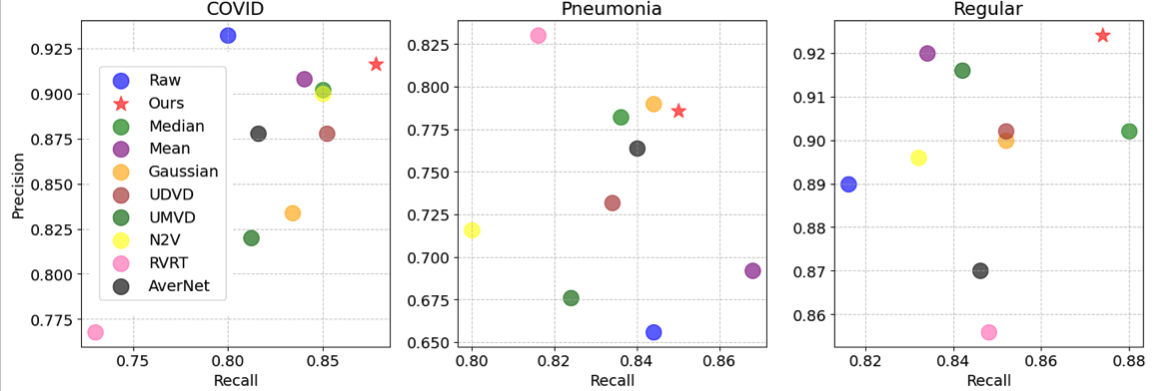
\includegraphics[width=\linewidth]{figs/class_POCUS_PR_all.jpg}
    \caption{\NAME{} (starred) has high precision and high recall across all POCUS classes.}
    \label{fig:classwise_POCUS}
\end{figure}

\section{Implementation Details}\label{sec:implementation_deets}

\subsection{\NAME{} Architecture Details}
Our method uses a series of convolution blocks with skip connections as an encoder $\Phi$, a bottleneck (hourglass network) $\Theta$, and a reconstruction decoder $\Psi$. Architectural details about each of these are shown in \cref{tab:denoiser_arch}. For more implementation details, the code is publicly available \href{https://github.com/suzanne-stathatos/SAVeD}{here}.

\begin{table*}[t]
    \centering
    \vspace{0pt} % Ensures top alignment
\begin{tabular}{l c c}
\toprule
\multicolumn{3}{c}{\textit{Encoder}}\\
    Type & Input shape & Output shape\\
    \hline\\
    \text{Conv\_block} & (1,1024,512) & (16, 1024, 512)\\
    Pooling & (16, 1024, 512) & (16, 512, 256) \\
    Skip & (16, 1024, 512) & (16, 512, 256) \\
    \text{Conv\_block} & (16, 512, 256) & (32, 512, 256) \\
    Pooling & (32, 512, 256) & (32, 256, 128) \\
    Skip & (32, 512, 256) & (32, 256, 128) \\
    \text{Conv\_block} & (32, 256, 128) & (64, 156, 128)\\
    Pooling & (64, 156, 128) & (64, 128, 64) \\
    Skip & (64, 156, 128) & (64, 128, 64) \\
    \text{Conv\_block} & (64, 128, 64) & (128, 128, 64)\\
    Pooling & (128, 128, 64) & (128, 64, 32)\\
    Skip & (128, 128, 64) & (128, 64, 32)\\
    \text{Conv\_block} & (128, 64, 32) & (256, 64, 32) \\
    Pooling & (256, 64, 32) & (256, 32, 16) \\
    Skip & (256, 64, 32) & (256, 32, 16) \\
    \text{Conv\_block} & (256, 32, 16) & (512, 32, 16) \\
    Pooling & (512, 32, 16) & (512, 16, 8) \\
    Skip & (512, 32, 16) & (512, 16, 8) \\    
\bottomrule
% \toprule
% \multicolumn{3}{c}{\textit{Bottleneck}}\\
% \bottomrule
\toprule
\multicolumn{3}{c}{\textit{Decoder}}\\
    Type & Input shape & Output shape\\
    \hline\\
    Upsample\_block & (512, 16, 8) & (256, 32, 16) \\
    Skip\_connect & (256, 32, 16) & (768, 32, 16) \\
    Conv\_block & (768, 32, 16) & (512, 32, 16)\\
    Upsample\_block & (512, 32, 16) & (256, 64, 32) \\
    Skip\_connect & (256, 64, 32) & (512, 64, 32)\\
    Conv\_block & (512, 64, 32) & (256, 64, 32) \\
    Upsample\_block & (256, 64, 32) & (128, 128, 64) \\
    Skip\_connect & (128, 128, 64) & (256, 128, 64) \\
    Conv\_block & (256, 128, 64) & (128, 128, 64) \\
    Upsample\_block & (128, 128, 64) & (64, 256, 128) \\
    Skip\_connect & (64, 256, 128) & (128, 256, 128) \\
    Conv\_block & (128, 256, 128) & (64, 256, 128) \\
    Upsample\_block & (64, 256, 128) & (32, 512, 256) \\
    Skip\_connect & (32, 512, 256) & (64, 512, 256) \\
    Conv\_block & (64, 512, 256) & (32, 512, 256) \\
    Upsample\_block & (32, 512, 256) & (1, 1025, 512) \\
\bottomrule
\end{tabular}    
    \caption{\textbf{Architecture details of the encoder, bottleneck, and decoder of \NAME{}.} ``\text{Conv\_block}" is a basic convolutional block composed of 3x3 convolution with padding side of 1 and ReLU activation. ``Skip" is a skip connection (stored to be input into the decoder) composed by maxpooling and then running a 1x1 convolution. ``Upsample\_block" is a 2D ConvTranspose with a 2x2 kernel and a stride of 2 and a ReLU activation. ``Skip\_connect'' is the concatenation of the output from Upsample\_block+Conv\_block and the ``Skip'' corresponding to the same layer saved by the encoder. Note that this architecture is on input size of 1024x512.}
    \label{tab:denoiser_arch}
\end{table*}

\begin{table*}[t]
    \centering
    \vspace{0pt} % Ensures top alignment
\begin{tabular}{l c c}
\toprule
\multicolumn{3}{c}{\textit{Encoder}}\\
    Type & Input shape & Output shape\\
    \hline\\
    \text{Conv\_block} & (3, 1024, 512) & (16, 1024, 512)\\
    Pooling & (16, 1024, 512) & (16, 512, 256) \\
    \text{Conv\_block} & (16, 512, 256) & (32, 512, 256) \\
    Pooling & (32, 512, 256) & (32, 256, 128) \\
    \text{Conv\_block} & (32, 256, 128) & (64, 156, 128)\\
    Pooling & (64, 156, 128) & (64, 128, 64) \\
    \text{Conv\_block} & (64, 128, 64) & (128, 128, 64)\\
    Pooling & (128, 128, 64) & (128, 64, 32)\\
    \text{Conv\_block} & (128, 64, 32) & (256, 64, 32) \\
    Pooling & (256, 64, 32) & (256, 32, 16) \\
    \text{Conv\_block} & (256, 32, 16) & (512, 32, 16) \\
    Pooling & (512, 32, 16) & (512, 16, 8) \\
\bottomrule
% \toprule
% \multicolumn{3}{c}{\textit{Bottleneck}}\\
% \bottomrule
\toprule
\multicolumn{3}{c}{\textit{Decoder}}\\
    Type & Input shape & Output shape\\
    \hline\\
    Bilinear\_upsample\_block & (512, 16, 8) & (512, 32, 16) \\
    Conv\_block & (512, 32, 16) & (256, 32, 16)\\
    Bilinear\_upsample\_block & (256, 32, 16) & (256, 64, 32) \\
    Conv\_block & (256, 64, 32) & (128, 64, 32) \\
    Bilinear\_upsample\_block & (128, 64, 32) & (128, 128, 64) \\
    Conv\_block & (128, 128, 64) & (64, 128, 64) \\
    Bilinear\_upsample\_block & (64, 128, 64) & (64, 256, 128) \\
    Conv\_block & (64, 256, 128) & (32, 256, 128) \\
    Bilinear\_upsample\_block & (32, 256, 128) & (32, 512, 256) \\
    Conv\_block & (32, 512, 256) & (16, 512, 256) \\
    Bilinear\_upsample\_block & (16, 512, 256) & (16, 1024, 512) \\
    Conv\_block & (16, 1024, 512) & (1, 1024, 512)\\
\bottomrule
\end{tabular}    
    \caption{\textbf{Architecture details of the vanilla autoencoder.} ``\text{Conv\_block}" is a basic convolutional block composed of 3x3 convolution with padding side of 1 and ReLU activation.  ``Bilinear\_upsample\_block" is a Bilinear Upsample kernel with a scale factor of 2 and align corners set to True. Note that this architecture is on input size of 1024x512.}
    \label{tab:autoencoder_arch}
\end{table*}

\subsection{\NAME{} Hyperparameter Comparisons}\label{sec:our_denoiser_hyperparams_and_details}
The hyperparameters for our method are in \cref{tab:hyperparams}. All DAE models are trained until the training loss converges on 2 NVIDIA RTX 4090 GPUs. 

\begin{table*}[t]
    \centering
    \resizebox{\textwidth}{!}{%
        \vspace{0pt} % Ensures top alignment
\begin{tabular}{l c c c c c c c c}
\toprule
Dataset & Resolution & Target & Epochs & Batch size & Learning Rate & Optimizer & Scheduler \\
\hline
CFC22 & (1024,512) & $S_{t,T=1}$ & 20 & 16 & 0.0005 & AdamW & Plateau f=0.1 pat=2 \\
POCUS & (1024,512) & $S_{t,T=1}$ & 120 & 8 & 0.0005 & AdamW & Step ss=2, $\gamma=0.05$\\
BUV & (1024,1024) & ${\text{inverse}(S_{t,T=1})}$ & 40 & 8 & 0.0005 & AdamW & Step ss=2, $\gamma=0.05$\\
Fluo & (1024,1024) & $I_t$ & 1000 & 8 & 0.0005 & AdamW & Step ss=2, $\gamma=0.05$\\
\bottomrule
\end{tabular}
    }
    \caption{\textbf{\NAME{} Hyperparameters.} Note ``$\text{inverse}(S_{t,T=1})$''$=\min(0, I_t - I_{t-T}) + I_t + \min(0, I_t - I_{t+T})$. f=Factor, pat=Patience, ss=Step size.}
    \label{tab:hyperparams}
\end{table*}

% \subsection{Denoiser Metric Details for CFC22}\label{sec:denoiser_metric_details}

\begin{figure}
    \centering
    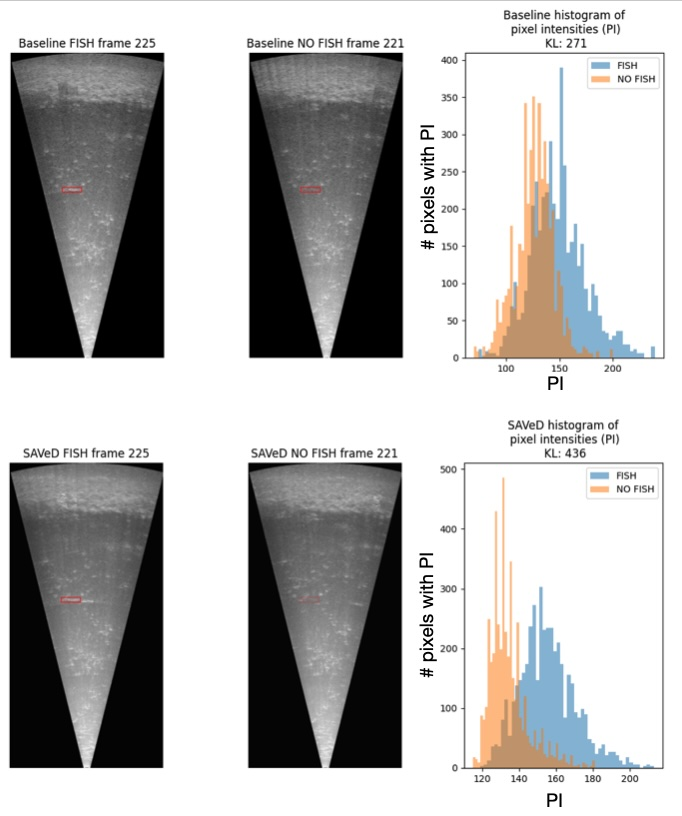
\includegraphics[width=\linewidth]{figs/detection_denoising_metric.jpg}
    \caption{\textbf{Visualization of $FBD$}. Both images on the left are noisy images. The image on the far left has a fish located in the red bounding box. The image in the middle is a frame from the same video clip but with no fish in the red box. The histogram compares the pixel intensity values of the pixels within the bounding boxes. We can see these distributions, while overlapping, are distinct.}
    \label{fig:denoiser_metric_details}
\end{figure}

\subsection{CFC22 Detector Details}\label{sec:cfc_detector_hyperparams}
We fine-tune a YoloV5-small model pretrained on COCO using the default training settings from Ultralytics over 5 epochs with a batch size of 16. As in \citet{cfc2022eccv}, we resize all inputs to have 896 pixels as their longest side; the learning rate is 0.0025. We select the best model checkpoint based on validation mAP$_{50}$. We train on two NVIDIA RTX A6000 GPUs. We recognize that the number of epochs (5) differs from the number of epochs in the original paper (150), and that is intentional. The reasoning is two-fold: 1.) CFC22++ Val and Test Performance after 5 epochs are $<1\%$ lower than Val and Test Performance after 150 epochs, therefore our denoised improvement beats the CFC22++ method also after CFC22++ is trained for 150 epochs while the detector model based on \NAME{} frames is trained for 5 epochs; 2.) We wanted to show that a very simple detector could be used as a result of passing in denoised frames. 



\begin{figure}[tp]
    \centering
    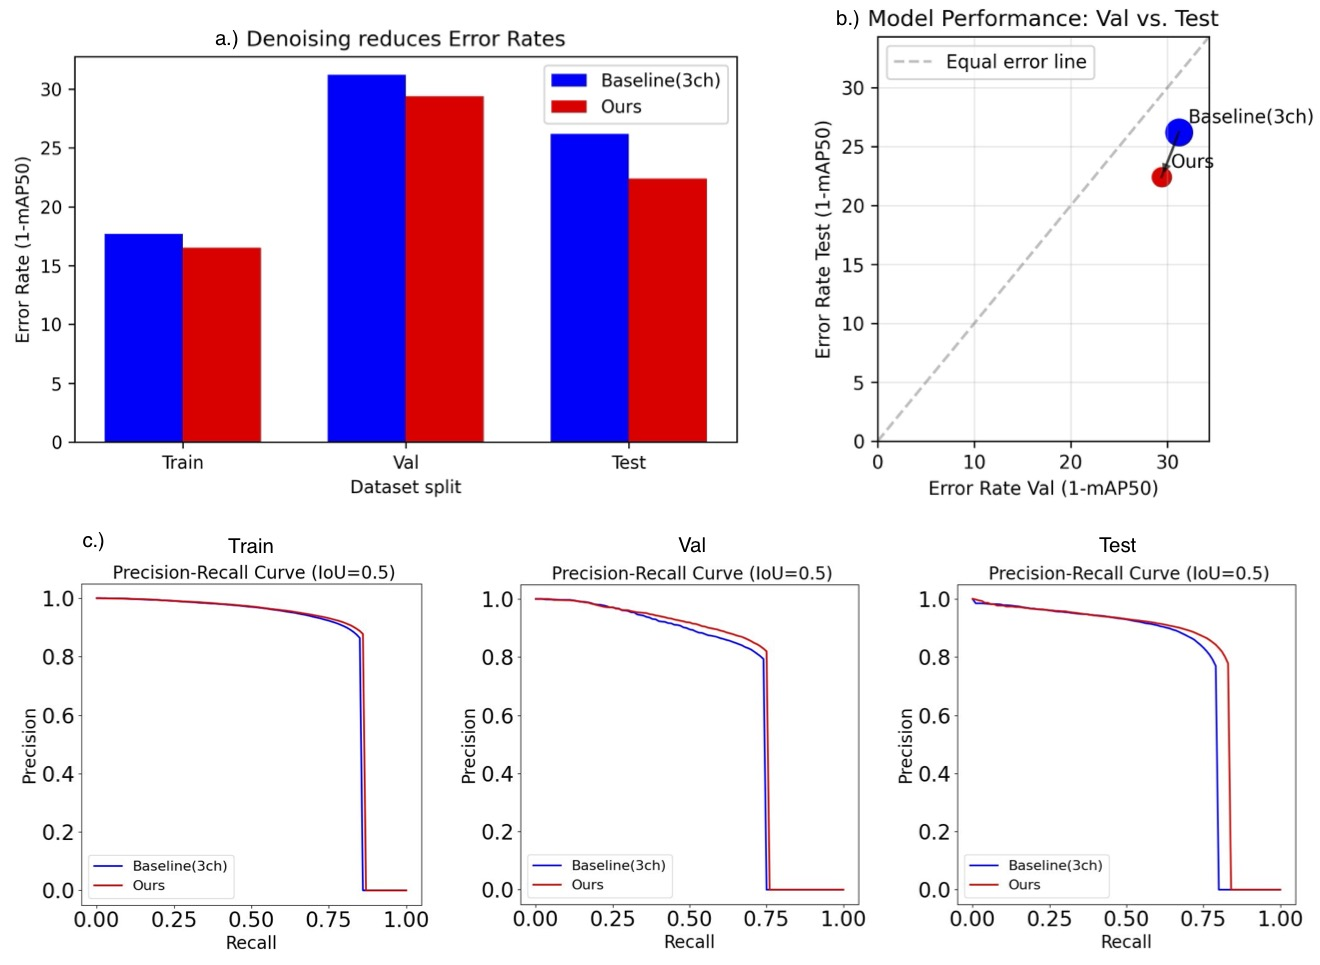
\includegraphics[width=\linewidth]{figs/error_rate_analysis.jpg}
    \caption{\textbf{Denoising lowers detections error-rates by improving precision and recall} (a) shows baseline detection error (1-mAP$_{50}$) compared to our detection error after our denoising preprocessing step. For all splits train, val, and test, denoising results in lower error. (b) compares error rates from the validation set (x-axis) to error rates from the test set (y-axis) to see how denoising impacts each split. There is a 5.8\% reduction in error in the val set and a 14.5\% reduction in error on the test set. (c) Shows inverted Precision-Recall plots for each CFC22 dataset split -- precision and recall both improve for all splits.}
    \label{fig:fig5}
    \vspace{1em} % Optional: Add some vertical space between the figure and table

    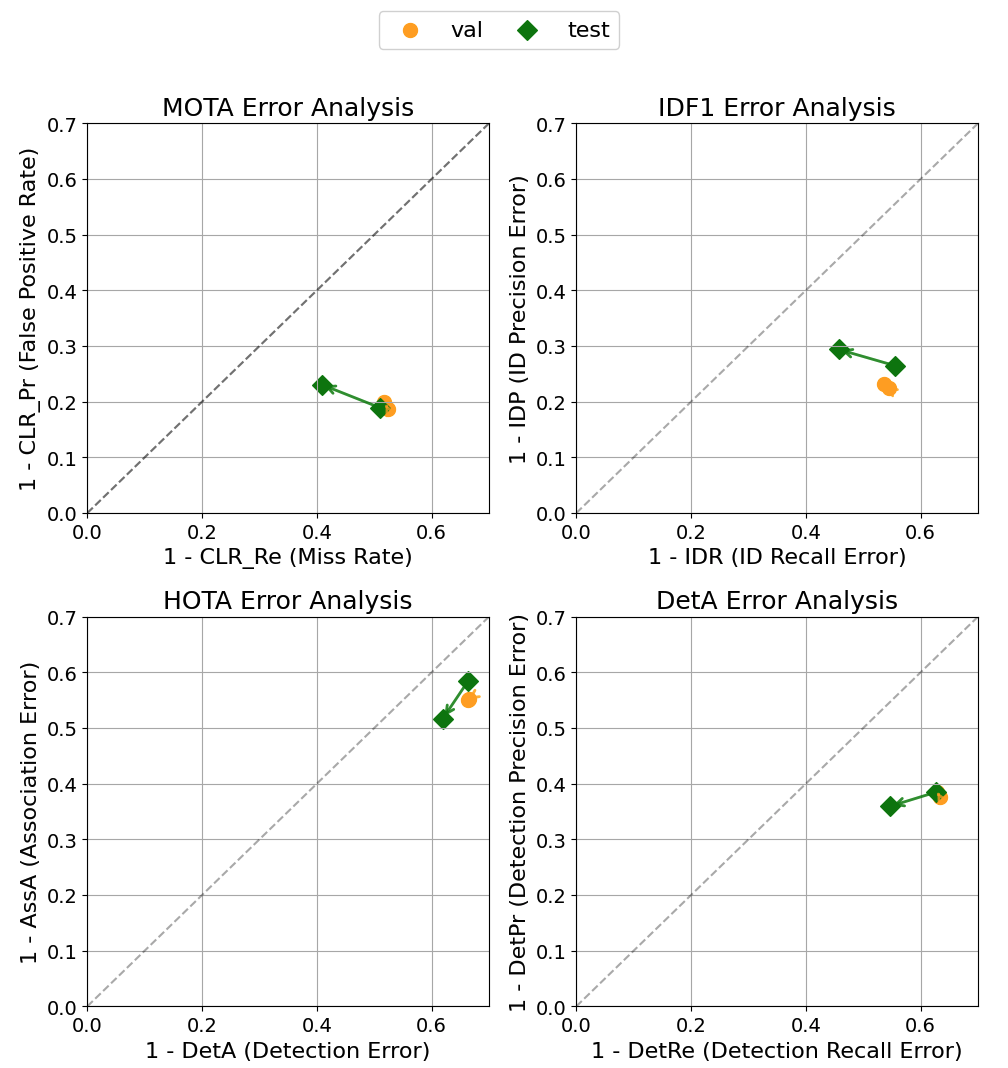
\includegraphics[width=\linewidth]{figs/track_perf_deepdive.jpg}
    \caption{\textbf{Breakdown of track performance improvements for CFC22 val and test}. We can see test improves far more than val, as is standard for the CFC22 dataset.}
    \label{fig:track_perf_deepdive}
\end{figure}

\subsection{CFC22 Tracker Details}\label{sec:cfc_tracker_hyperparams}
We use a pretrained ByteTrack tracker with hyperparameters selected as the optimal hyperparameters for tracking performance on the validation set. Max age, the time until a missing or occluded object is assigned a new id, is 20; Min hits, the minimum number of frames with a track for the track to be considered valid, is 11; IOU threshold, the iou required for an object to be considered the same in the subsequent frame, is 0.01.

\section{Visualizations}\label{sec:visualizations}
Additional visualizations of the denoising performance on fish in sonar (CFC22\cite{cfc2022eccv})
% and ultrasound health (POCUS\cite{born2021accelerating, born2021l2}, BUV\cite{CVANet})
can be seen in \cref{fig:additional_fish_denoised}).

\begin{figure}[htbp]
    \centering
    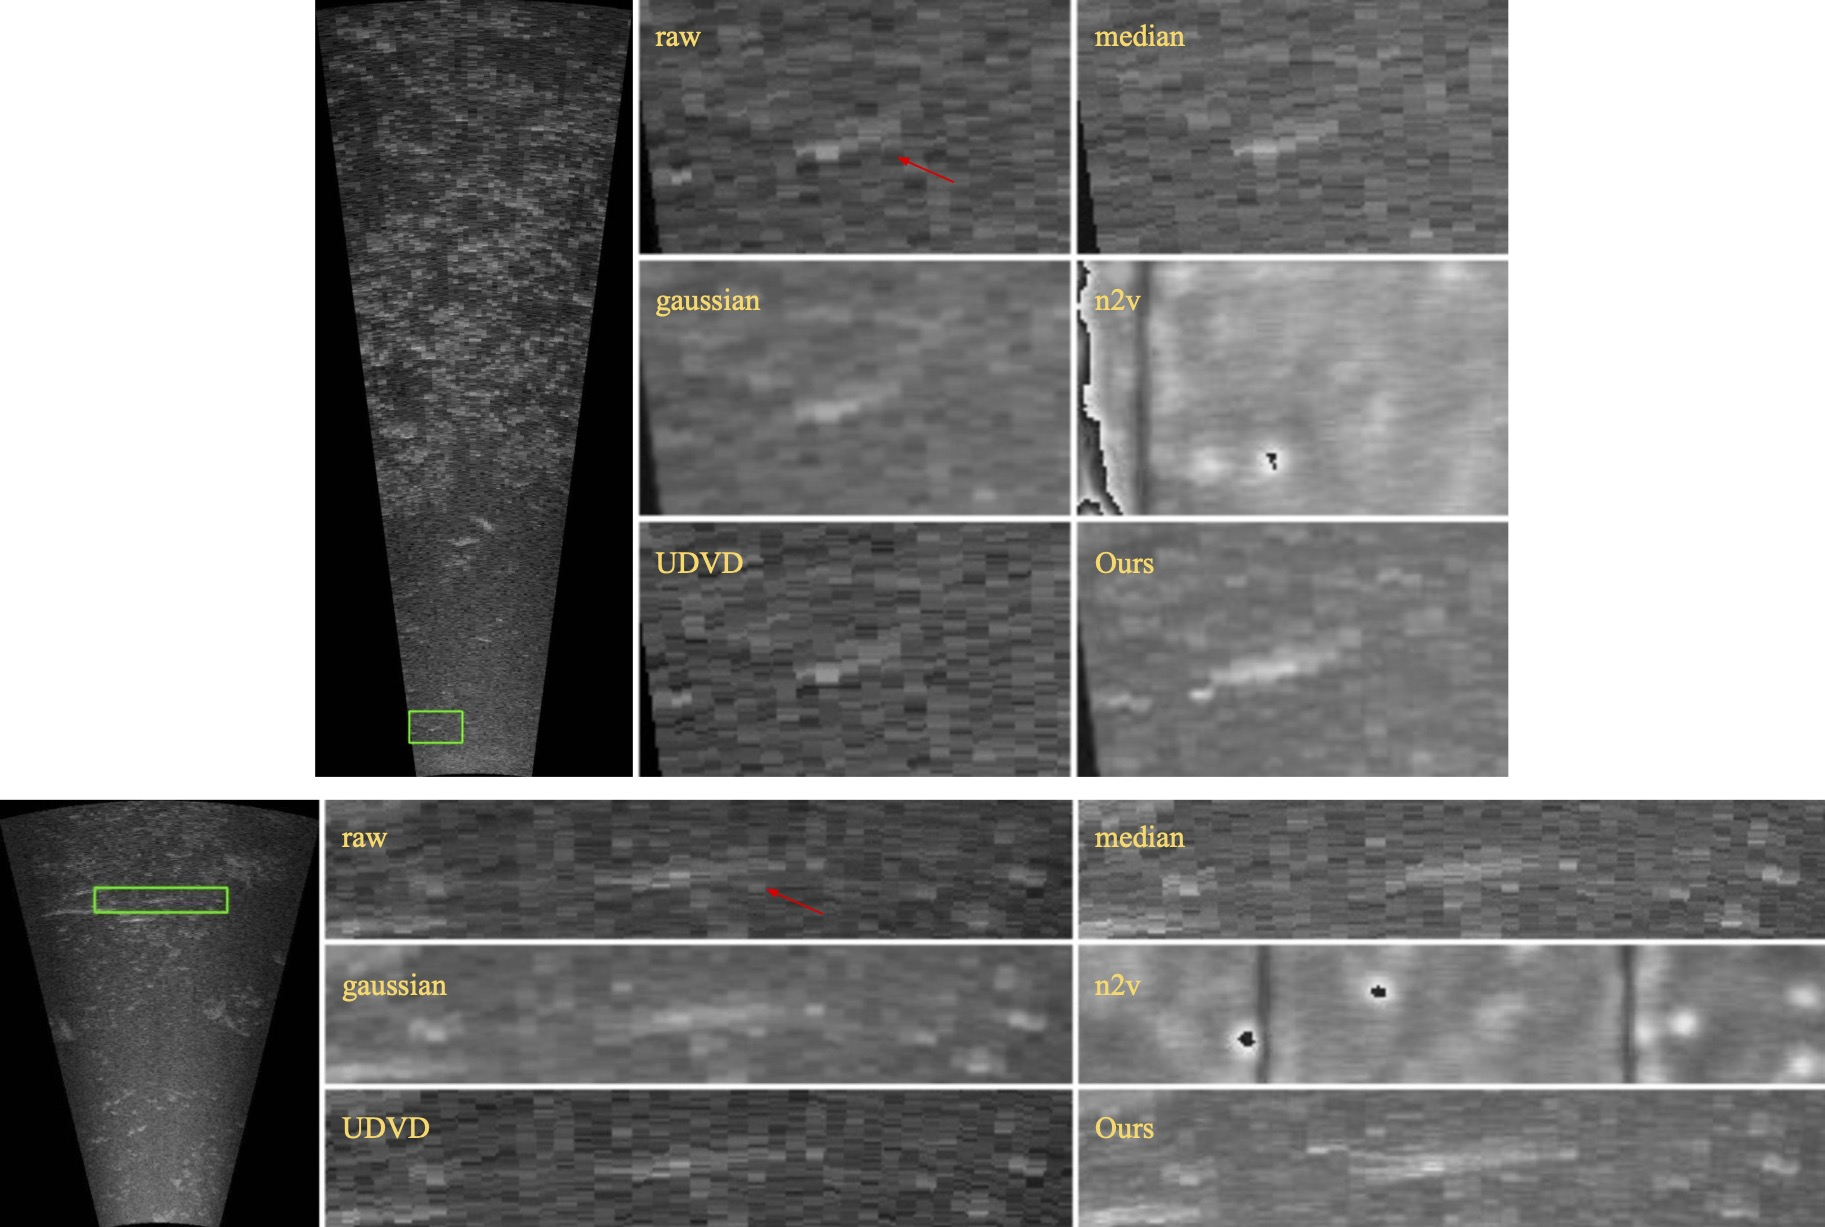
\includegraphics[width=\linewidth]{figs/fish_qual_denoising_supp.jpg}
        % \caption{Subfigure 1} % Optional: Add captions for each subfigure
        % \label{fig:subfig1}
    \caption{\textbf{Additional visualizations of denoising methods on CFC22}}
    \label{fig:additional_fish_denoised}
\end{figure}

% \begin{figure}[H]
%     \centering
%     \includegraphics[width=\linewidth]{figs/Qualitative_denoising_POCUS.jpg}
%     \caption{\textbf{Additional visualizations of denoising methods on POCUS}}
% \end{figure}

\begin{figure}[htbp]
    \centering
    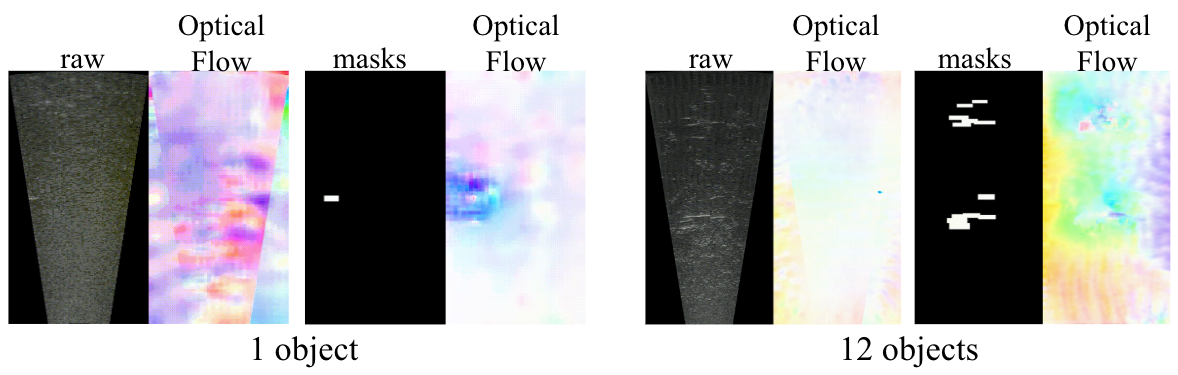
\includegraphics[width=\linewidth]{figs/RAFT_on_cfc_h.png}
    \caption{\textbf{RAFT \cite{teed2020RAFT} on CFC22 imagery and bounding box masks.} On the left, we can see the optical flow signal does not find the fish. When looking at the motion from the bounding-box mask of the fish (making the background movement stationary), the optical flow signal area is far greater than the actual area of the fish. On the right are frames (with fish and corresponding bounding-box masks), when there are 12 fish in the frame at once. Again, optical flow's signal is weak with the fish movement compared to the background. With the mask movement, optical flow signals cluster in groups of masked fish, but individuals are difficult to distinguish.}
    \label{fig:RAFT_on_cfc}

\end{figure}